% THIS IS SIGPROC-SP.TEX - VERSION 3.1
% WORKS WITH V3.2SP OF ACM_PROC_ARTICLE-SP.CLS
% APRIL 2009
%
% It is an example file showing how to use the 'acm_proc_article-sp.cls' V3.2SP
% LaTeX2e document class file for Conference Proceedings submissions.
% ----------------------------------------------------------------------------------------------------------------
% This .tex file (and associated .cls V3.2SP) *DOES NOT* produce:
%       1) The Permission Statement
%       2) The Conference (location) Info information
%       3) The Copyright Line with ACM data
%       4) Page numbering
% ---------------------------------------------------------------------------------------------------------------
% It is an example which *does* use the .bib file (from which the .bbl file
% is produced).
% REMEMBER HOWEVER: After having produced the .bbl file,
% and prior to final submission,
% you need to 'insert'  your .bbl file into your source .tex file so as to provide
% ONE 'self-contained' source file.
%
% Questions regarding SIGS should be sent to
% Adrienne Griscti ---> griscti@acm.org
%
% Questions/suggestions regarding the guidelines, .tex and .cls files, etc. to
% Gerald Murray ---> murray@hq.acm.org
%
% For tracking purposes - this is V3.1SP - APRIL 2009

\documentclass{acm_proc_article-sp}
\usepackage{graphicx}
\usepackage{subfigure}
\usepackage{multirow}
\graphicspath{{pics/}}

\begin{document}

\title{Expose and Adjust Parameters of General Purpose Memory Allocator}
%
% You need the command \numberofauthors to handle the 'placement
% and alignment' of the authors beneath the title.
%
% For aesthetic reasons, we recommend 'three authors at a time'
% i.e. three 'name/affiliation blocks' be placed beneath the title.
%
% NOTE: You are NOT restricted in how many 'rows' of
% "name/affiliations" may appear. We just ask that you restrict
% the number of 'columns' to three.
%
% Because of the available 'opening page real-estate'
% we ask you to refrain from putting more than six authors
% (two rows with three columns) beneath the article title.
% More than six makes the first-page appear very cluttered indeed.
%
% Use the \alignauthor commands to handle the names
% and affiliations for an 'aesthetic maximum' of six authors.
% Add names, affiliations, addresses for
% the seventh etc. author(s) as the argument for the
% \additionalauthors command.
% These 'additional authors' will be output/set for you
% without further effort on your part as the last section in
% the body of your article BEFORE References or any Appendices.

\numberofauthors{3} %  in this sample file, there are a *total*
% of EIGHT authors. SIX appear on the 'first-page' (for formatting
% reasons) and the remaining two appear in the \additionalauthors section.
%
\author{
% You can go ahead and credit any number of authors here,
% e.g. one 'row of three' or two rows (consisting of one row of three
% and a second row of one, two or three).
%
% The command \alignauthor (no curly braces needed) should
% precede each author name, affiliation/snail-mail address and
% e-mail address. Additionally, tag each line of
% affiliation/address with \affaddr, and tag the
% e-mail address with \email.
%
% 1st. author
\alignauthor Fan Wu\\
       \affaddr{Department of Computer Science, UCL}\\
       \affaddr{Gower Street}\\
       \affaddr{London WC1E 6BT, United Kingdom}\\
       \email{fan.wu.12@ucl.ac.uk}
% 2nd. author
\alignauthor Mark Harman\\
       \affaddr{Department of Computer Science, UCL}\\
       \affaddr{Gower Street}\\
       \affaddr{London WC1E 6BT, United Kingdom}\\
       \email{mark.harman@ucl.ac.uk}
% 3rd. author
\alignauthor Yue Jia\\
       \affaddr{Department of Computer Science, UCL}\\
       \affaddr{Gower Street}\\
       \affaddr{London WC1E 6BT, United Kingdom}\\
       \email{yue.jia@ucl.ac.uk}
}
% There's nothing stopping you putting the seventh, eighth, etc.
% author on the opening page (as the 'third row') but we ask,
% for aesthetic reasons that you place these 'additional authors'
% in the \additional authors block, viz.
% Just remember to make sure that the TOTAL number of authors
% is the number that will appear on the first page PLUS the
% number that will appear in the \additionalauthors section.

\maketitle
\begin{abstract}
Abstract here
\end{abstract}

% A category with the (minimum) three required fields
\category{H.4}{Information Systems Applications}{Miscellaneous}
%A category including the fourth, optional field follows...
\category{D.2.8}{Software Engineering}{Metrics}[complexity measures, performance measures]

\terms{Theory}

\keywords{Parameter tuning, parameter exposure, dynamic memory allocator} % NOT required for Proceedings

\section{Introduction}
Introduction to the background of non-functional requirements. Motivation. Brief introduction of experiments and result.

\section{Background}
Introduction to several basic memory allocation strategies. Description of dlmalloc. Could be modified from my first year report section 2.1 and 3.1.
\subsection{Allocation Strategies}
\label{sec_allocationstrategies}
When an application asks for some memory from the operating system, the simplest way is to give exact size of memory it requests, and to return that memory back to the system when the application frees it. However, getting memory from the system and returning it to the system usually require invoking some system calls, which are much slower than other operations. Plus memory allocation and deallocation are very basic and used frequently in most of the applications, so frequently allocating memory directly from the system is impractical. Memory allocators have risen to solve this problem using different allocation strategies. They usually are the only one who communicate with the operating system in terms of memory in any application. They apply memory from the system, hold some extra available memory and manage them in order to respond to any memory request from the application as efficiently as possible. The freed memory is not returned to the system but handled by memory allocators and then given back to system by the allocator when it is necessary. Different ways of memory management significantly influence the performance of an application and researchers have proposed and studied many of them.

In terms of allocation strategies, many researchers have proposed many different strategies for memory allocation and deallocation, which have been well studied and have their own strength and disadvantages\cite{memoryallocatorreview1995}. The basic data structure that most of the allocation strategies use is a linked list of free chunks of memory, which uses a little overhead to store some basic information such as the size of the chunk and whether it is in use, whilst using the free chunk itself to keep the linking pointers. The linked list is also called free list since it only links the unoccupied chunks. Whenever the application issues a memory request, the allocator searches the free list to find a free chunk that meets the request and removes it from the list. When a chunk is freed by the application, it won't be returned to the operating system immediately but inserted to the free list in case the application may soon request a chunk in the same size. A simple example of a free list is depict in Figure \ref{fig_1}, in which the shaded regions represent occupied memory chunks.
\begin{figure}[htbp]
\centering
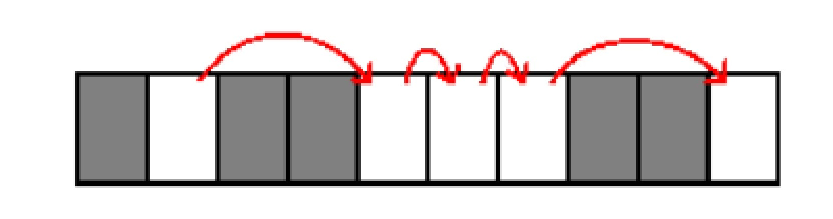
\includegraphics[width=1.5in]{fig1}
\caption{Basic Linked List}\label{fig_1}
\end{figure}

\textbf{Sequential fit} is a set of similar allocation strategies including first fit, next fit and best fit. They all use no more than a double linked list to manage the free chunks. When a memory request comes, first fit starts searching the list from the beginning and stops at the first time it meets a free chunk that fulfills the request. It splits the free chunk into two pieces, one of which is in the request size and returned to the application whilst the remainder is inserted back to the list. One big disadvantage of first fit is poor locality, which increases the possibility of cache miss, thus increases the reference time as well as the total running time. Next fit also searches the free list one by one, but starting from where it finds the free chunk for the previous request. The first and next fit both continuously split large free chunks to smaller ones, which cannot be used for later large request, so they both suffer from big fragmentation. The best fit, on the other hand, goes through the whole free list before it makes a decision. So it guarantees to return the smallest free chunk in the list that meets the request, sometimes even the exact fit, hence it performs better in terms of fragmentation than first fit and next fit\cite{Johnstone:1998:MFP:301589.286864}. However, because it goes through the whole list every time there is a request, it costs a lot of time for allocation especially when the free list is very long.

\begin{figure}[htbp]
\centering
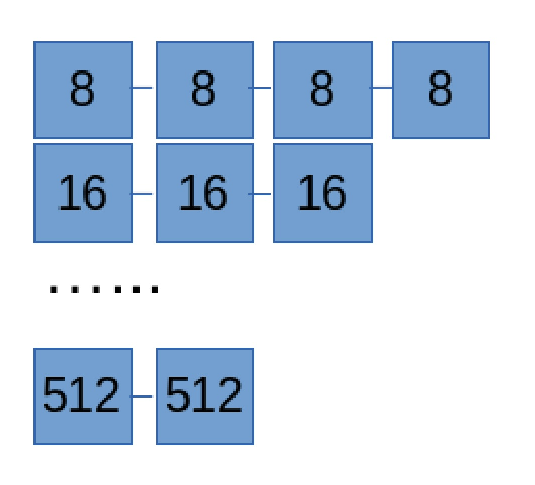
\includegraphics[width=1in]{fig2}
\caption{Segregated free lists}\label{fig_2}
\end{figure}
\textbf{Segregated fit} keeps multiple free lists at the same time (Figure \ref{fig_2}) instead of managing one free list like what sequential fit does. Each of the free lists kept by segregated fit policy contains free chunks in the exact same size which is always a multiple of 8 bytes or a size in power of 2. This has also been known to increase the internal fragmentation (see section \ref{sec_fragmentation}). Each time there is a request of size \emph{n}, it only needs to fetch a free chunk from one of the free lists that corresponds to size \emph{n}. So it saves the allocation time by diminishing the searching time for a best fit whilst keeping a low fragmentation. But it harms a little of the deallocation time since it has to find the exact free list in the deallocated size before the freed chunk can be inserted to that list. What's more, it is possible that there is no available free chunk in the free list that corresponds to the request size, in which case the allocator will get a larger chunk from the next non-empty free list and split the chunk to meet the request. A variant of segregated fit differs only on returning a free chunk without aplitting it even if the chunk is much bigger than the request size. In this allocation strategy, the memory consumption is much higher because each chunk is in a fixed size and may be serving a much smaller request so that the extra size in that chunk can not be reused by other requests. But there is no denying this simplified segregated fit strategy is fast. This also shows there is clearly a trade-off between allocation time and memory consumption.

\textbf{Coalescing} is a strategy which can be combined with or applied to the above allocation strategies, so can the ones introduced later. In order to save memory, most of the policies above choose to split a chunk before returning it to the application. This leads to more and more small chunks that cannot be used for big request. But some of these small chunks could be contiguous in the address space so that they can be concatenated to serve large request, in order to save memory. Coalescing policies try to concatenate contiguous free chunks into a bigger one, but when to apply coalescing remains adjustable in different allocators. This is because if an application request a chunk with size of \emph{n} right after it frees a chunk in the same size, the allocator may have coalesced the freed chunk but split it out from the concatenated chunk again to serve the same-size-request, which is a waste of computation. So instead of coalescing every time the application frees a chunk, some allocators apply coalescing in a fix frequency or once there is no big enough chunk that meets the request. In summary, whether the coalescing policy improves or diminishes the performance of an allocator really depends on the allocator itself and the allocation pattern of the application.

\textbf{Searching strategy} refers to how an allocator manages and searches the free list(s). Some allocators keep the free list(s) in ascending or descending order in terms of address or size. It is quick for searching but may cause poor locality. Good locality refers to trying to allocate chunks that may be accessed subsequently in the application, on the same physical page, in order to minimize the cache misses in the operating system as a means of saving execution time. Searching strategy is quite influential to locality since it determines where subsequent requests should be located. On the other hand, when a chunk is freed and returned to the allocator, there are several ways to place it back in the free list(s), two of which are first-in-first-out (FIFO) and last-in-first-out (LIFO). FIFO strategy gives the most recently released chunk the least priority and places it at the end of the searching queue, whilst LIFO gives the most recently released chunk the highest priority so that it is more likely to be reused in a short time. There is no telling which one is better since it depends on other allocation strategies and the application itself.

\textbf{Bitmap} is another combinable strategy that uses boolean flags to keep the status of chunks or free lists. When it stores the status of chunks, one bit usually represents whether a chunk is in use, and when it keeps the status of free lists, it usually means whether a free list is empty. The bitmap is designed to help the allocator to find an available chunk easily. It narrows the range down by searching the bitmap before searching a free chunk that meets the request.

\textbf{Buddy system} is a well known algorithm which involves a special splitting mechanism. It always allocates memory in several fixed sizes and whenever it needs to split a chunk into two, it splits it in a fixed ratio repeatedly until it meets the smallest chunk that bigger than the request size. In this special splitting mechanism coalescing is fast because finding the other ``buddy'' generated from the same splitting is no more than a couple of simple mathematical computation. Even though the splitting ratio is adjustable, buddy systems still suffer from huge internal fragmentation.

\subsection{Internal and External Fragmentation}
\label{sec_fragmentation}
Most of the memory allocators keep all the chunks in the size of multiple of 8 bytes due to the operating system requirements. In these cases, all the memory requests from applications are rounded up to an alignment of 8 bytes before they are really allocated. So the returned chunk is always equal to or slightly bigger than the request size without the applications being aware of it. Then the little extra padding memory is neglected and cannot be used by the applications. This is always refered to as internal fragmentation. On the other hand, at any point of a running application, the memory allocator always hold some free chunks instead of returning them to the operating system, so that it can quickly respond to some memory request from the application using these free chunks. And some of these free chunks may be too small to serve bigger request and for some reason they cannot be coalesced neither (e.g., not next to any other free chunks). The number of these small chunks may increase when the application proceeds, which causes the application occupying more memory than it really needs. This is also known as external fragmentation. 

Allocators always introduce fragmentation, in different degrees. Despite many attempts to minimize memory fragmentation in an efficient way, there is clearly a trade-off between running time and memory fragmentation. For instance allocators with coalescing policies reuse small free chunks by concatenating them whilst introducing more computation for coalescing. And both segregated fit and buddy systems suffer from high fragmentation but they always contribute to fast allocators. 

\subsection{\emph{Dlmalloc}}
\label{sec_dlmalloc}
\emph{Dlmalloc} keeps two set of segregated lists for small and large size requests respectively. 
\begin{figure}[htbp]
\centering
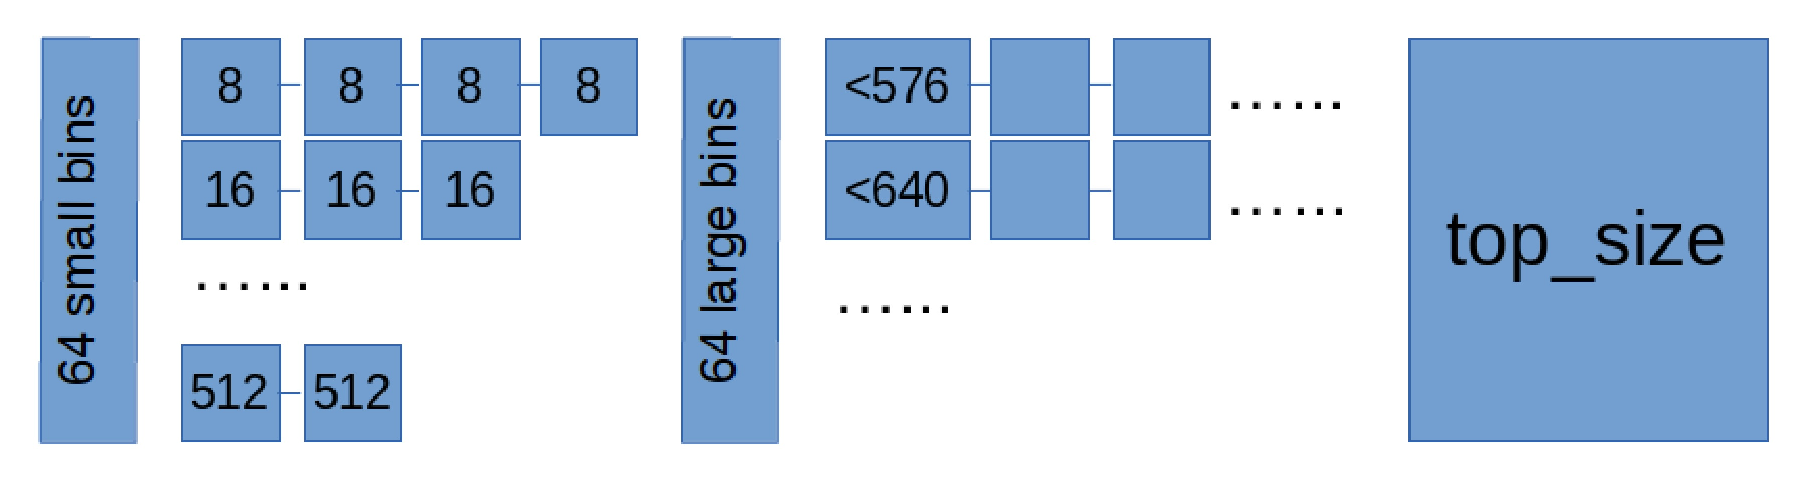
\includegraphics[width=0.4\textwidth]{fig7}
\caption{structure of \emph{dlmalloc}}\label{fig_7}
\end{figure}
Each of the segregated lists is called a bin and there are 64 small bins and 64 large bins in \emph{dlmalloc} (Figure \ref{fig_7}). For small bins, each one contains chunks in the same size aligned to multiple of 8 bytes, which makes the largest chunk in small bins 512 bytes. Since chunks in the same small bin are in the exact same size, there is no need to sort the list, and insertion to or deletion from the list is very quick. For large bins, each bin is associated with a range of size which doesn't overlap with that of other bins. All the chunks larger than 512 bytes are stored in one of the large bins according to its size and kept in ascending order. So finding a chunk with a desired size requires a thorough search of an associated bin in the worst case. Apart from these segregated lists, \emph{dlmalloc} also keeps a top chunk, which is always at the end of the heap so that it can be extended or shrinked without affecting the data structure of other bins. The top chunk is used only when there is no available chunk in any bins that meets the memory request.

\begin{figure}[htbp]
\centering
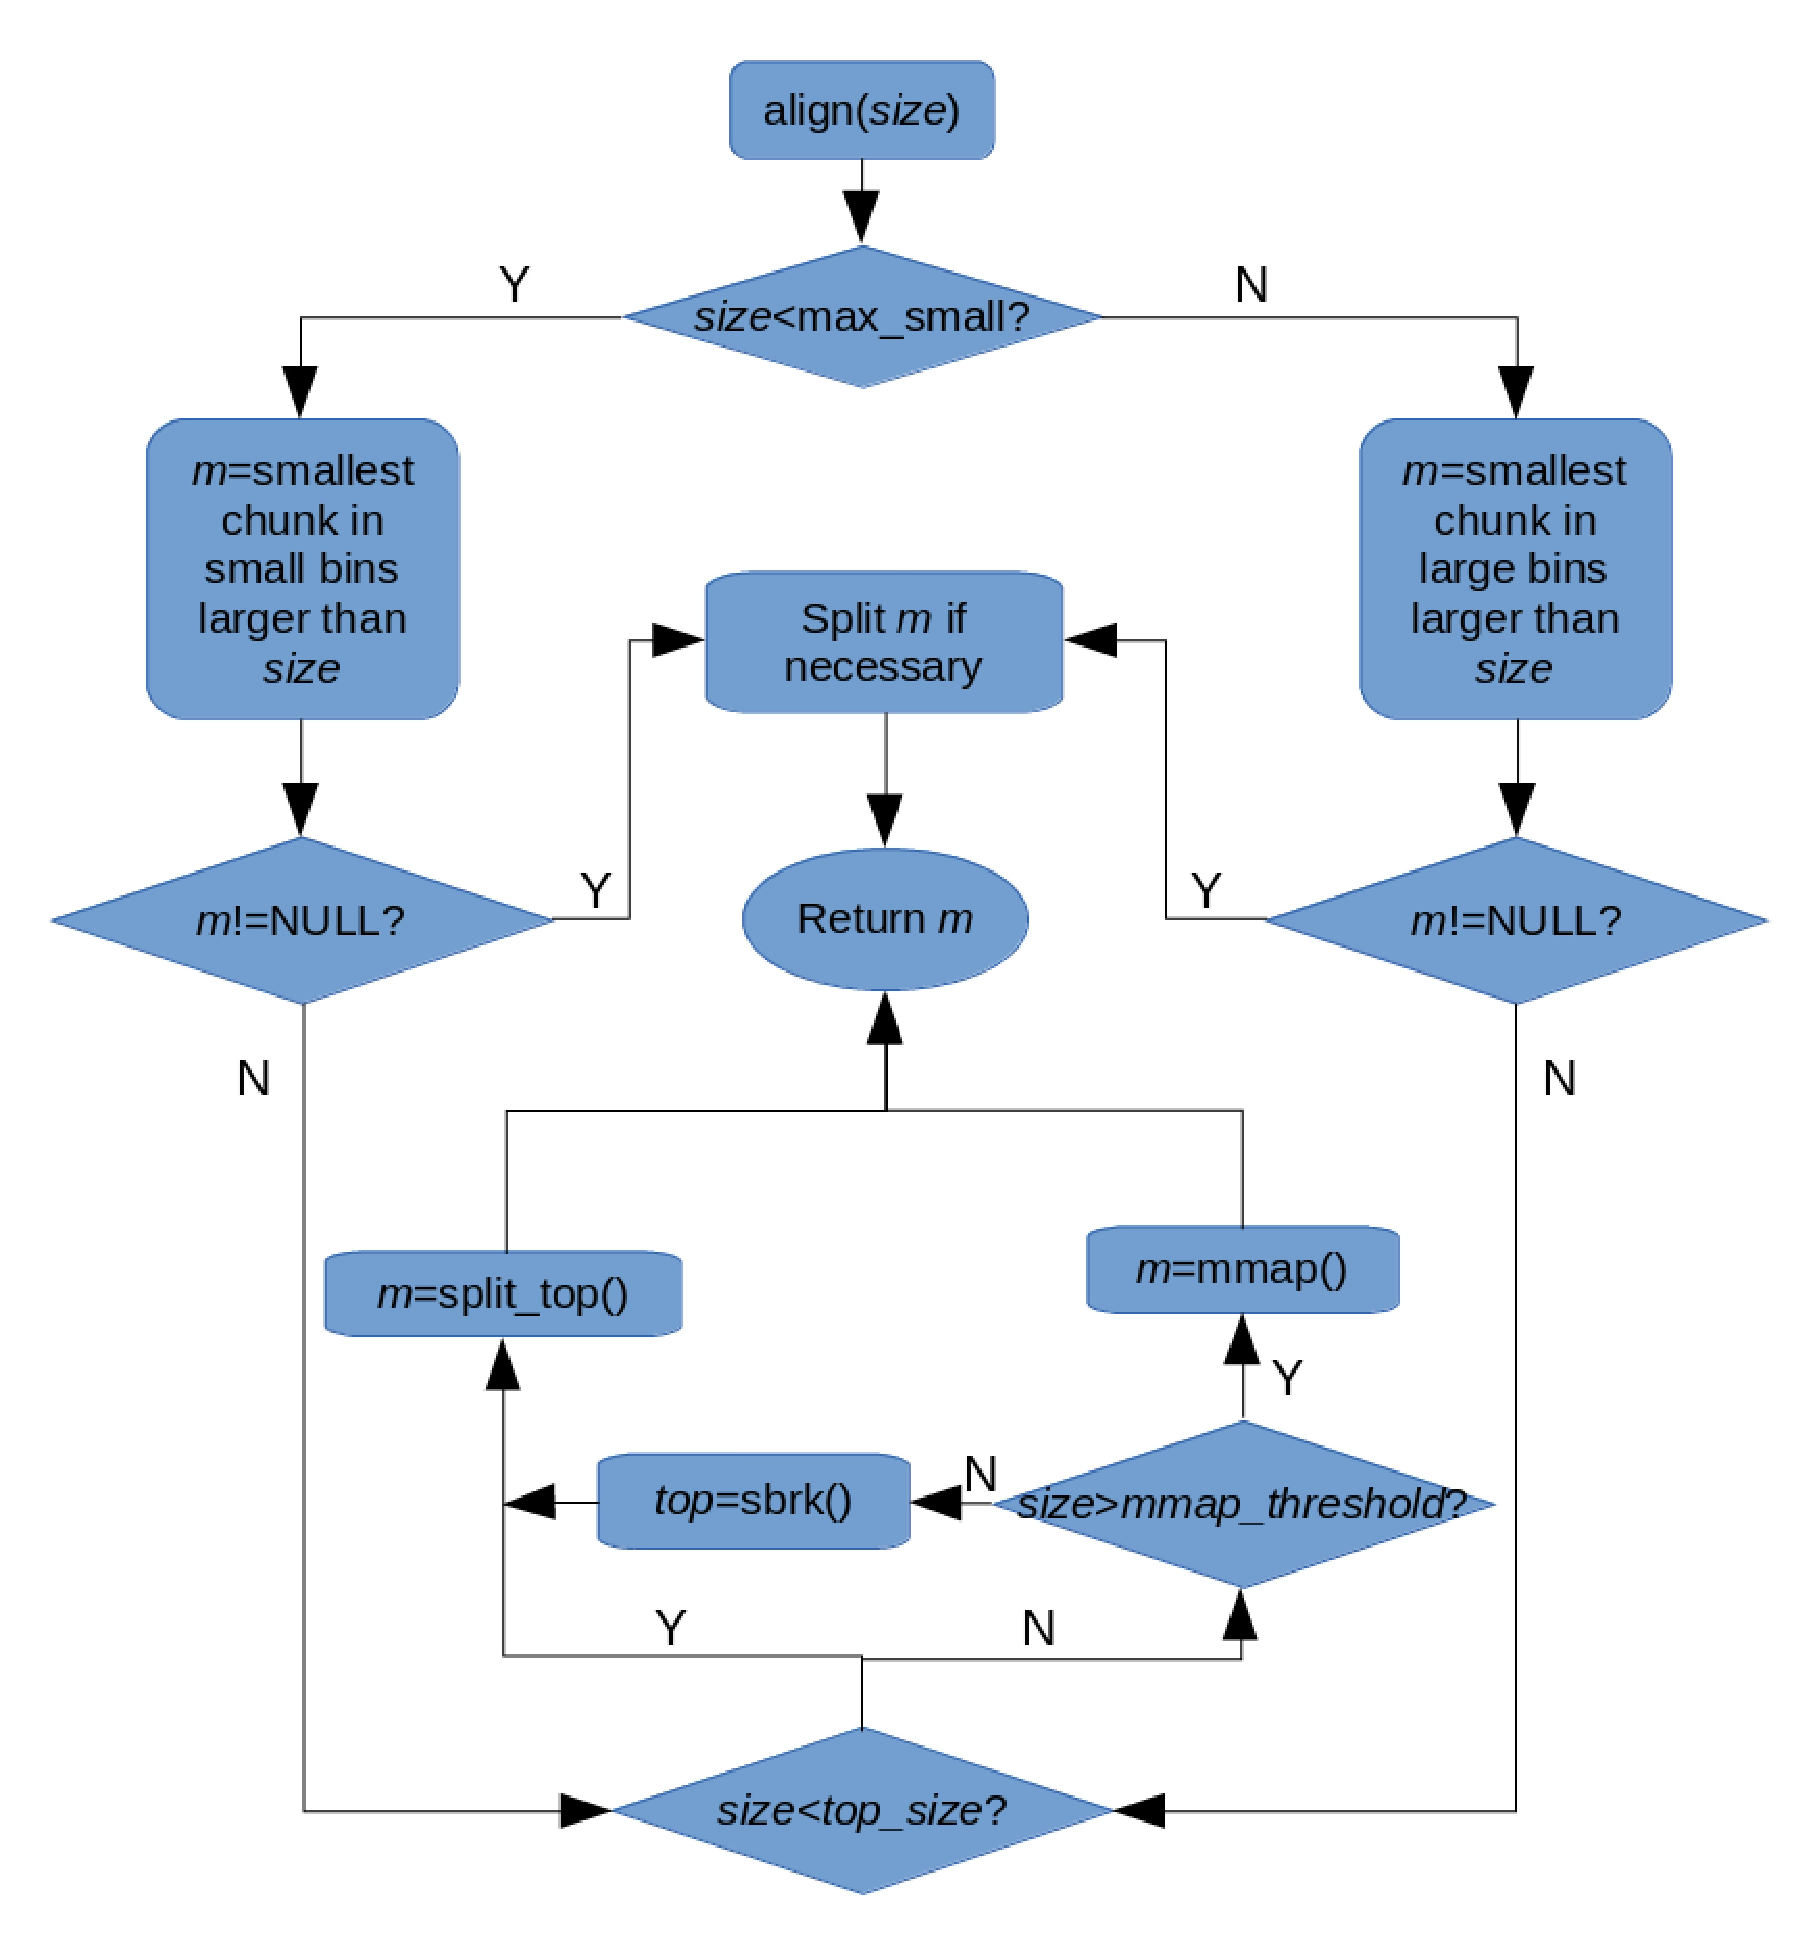
\includegraphics[width=0.4\textwidth]{fig8}
\caption{allocation process of \emph{dlmalloc}}\label{fig_8}
\end{figure}
When a memory request from the application comes, \emph{dlmalloc} first rounds it up to a multiple of 8 bytes, then determine whether it belongs to small or large bins(Figure \ref{fig_8}). Either way, it searches the corresponding bin(s) based on the request size. If an available chunk that meets the requirement is found, it is returned to the application before which split may be applied if necessary. Otherwise, \emph{dlmalloc} tries to use the top chunk to serve the request by splitting the top chunk if the request size is smaller than the size of the top chunk, in which case the remainder is preserved as the new top chunk. If the request size is too large to be gotten from the top chunk, \emph{dlmalloc} uses an \emph{mmap}-like system call to allocate this size of memory from the operating system directly only when the request size is bigger than a pre-defined threshold. Otherwise it tries to extend the top chunk using \emph{sbrk}-like system call, so that the extended top chunk is big enough to cover the request.
When a chunk is freed by the application, it is put back to one of the bins according to its size, after which \emph{dlmalloc} occasionally coalesces contiguous free chunks to create bigger chunks. If the top chunk is enlarged by combining free chunks next to it, it is also checked whether it is too large for the need of the application, in which case the top chunk may be shrinked. If the freed chunk was mapped directly from the system, it is released to system immediately. 
There are several other details and techniques in \emph{dlmalloc} that are less relevant to our work, so we don't list them in this article. But they can be easily found in \emph{dlmalloc}'s source code.

\section{Methods}
Introduction of the methods proposed in this paper. Including parameter tuning, sensitivity analysis via mutation operators, parameter exposure. Research Questions.

\section{Experiment Setup}
\subsection{Basic Parameters}
introduction to the existing tunable parameters in the original dlmalloc which are tuned in this work.

As a general-purpose allocator, \emph{dlmalloc} provides several tunable parameters to programmers to adjust at compilation. These parameters are defined as macros in the source code of \emph{dlmalloc}, but can be changed by compilers (we achieve that through \emph{gcc}'s ``-D'' flag in this work). In this article, we choose some of these parameters that are more likely to influence the allocator's behavior in terms of memory consumption, as our ``victims'', which are introduced as follows.

\textbf{MALLOC\_ALIGNMENT} is one of the most basic macros in \emph{dlmalloc}, representing a multiple of how many bytes all request sizes should be rounded up to. Most of other macros in \emph{dlmalloc} rely on this alignment to avoid any incompatibility. Its default value is $2*sizeof(void*)$ where $sizeof(void*)$ varies across different systems. 
\begin{table*}[htbp]
\centering
\caption{\emph{dlmalloc} parameters}
\label{tab_1}
\resizebox{0.8\textwidth}{!}{
\begin{tabular}{c|c|c|c|c}
\hline
macro & default & minimum & maximum & type \\
\hline
MALLOC\_ALIGNMENT & $2*sizeof(void*)$ & $sizeof(void*)$ & $16*sizeof(void*)$ & $2^n*sizeof(void*)$ \\
\hline
FOOTERS & \emph{false} & \emph{false} & \emph{true} & boolean \\
\hline
INSECURE & \emph{false} & \emph{false} & \emph{true} & boolean \\
\hline
NO\_SEGMENT\_TRAVERSAL & \emph{false} & \emph{false} & \emph{true} & boolean \\
\hline
MORECORE\_CONTIGUOUS & \emph{true} & \emph{false} & \emph{true} & boolean \\
\hline
DEFAULT\_GRANULARITY & 0 & 4KB & 512KB & $2^n$KB or 0 \\
\hline
DEFAULT\_TRIM\_THRESHOLD & 2048KB & 64KB & 16MB & $2^n$KB \\
\hline
DEFAULT\_MMAP\_THRESHOLD & 256KB & 16KB & 2MB & integer \\
\hline
MAX\_RELEASE\_CHECK\_RATE & 4095 & 1000 & 10000 & integer \\
\hline
TOP\_FOOT\_SIZE & 80B & 16B & 2KB & integer \\
\hline
\end{tabular}}
\end{table*}
The legitimate values for MALLOC\_ALIGNMENT are a power of 2 times $sizeof(void*)$ and we constrain the searching space from $sizeof(void*)$ to $16*sizeof(void*)$. The default value and searching range of MALLOC\_ALIGNMENT, as well as other macros, is given in Table \ref{tab_1}.

\textbf{FOOTERS}, \textbf{INSECURE} and \textbf{NO\_SEGMENT\_TRAVERSAL} are all boolean parameters. FOOTERS allows \emph{dlmalloc} place extra checking and dispatching information at the end of allocated chunks, which may increase memory consumption. The default value for FOOTERS is \emph{false}. When INSECURE is \emph{true}, \emph{dlmalloc} skips checks for usage errors and heap space overwrites. Its default value is \emph{false}, meaning \emph{dlmalloc} always keeps checking violated chunks by default. NO\_SEGMENT\_TRAVERSAL disables merging of segments that are contiguous and selectively releasing them to the OS if unused, by suppressing traversals of memory segments at some points of execution. It is set to \emph{false} by default. 

\textbf{DEFAULT\_GRANULARITY} is the unit for allocation and deallocation from the system. Large DEFAULT\_GRANULARITY tends to lead to higher memory consumption but lower allocation time. Normally it is set to the page size if the system supports contiguous \emph{sbrk}-like system call. It should have a value of power of 2 and at least one page size. By default it is set to 0 meaning it equals to the page size according to the system. When \textbf{MORECORE\_CONTIGUOUS} is \emph{true}, change of DEFAULT\_GRANULARITY is turned off and 0 is set for DEFAULT\_GRANULARITY.

\textbf{DEFAULT\_TRIM\_THRESHOLD} defines when the allocator should return some memory back to the system if it holds too much free memory. It only applies on the top chunk since allocation and deallocation from the system can only happen at the end of heap where the top chunk locates. If the allocator finds the size of the top chunk is bigger than DEFAULT\_TRIM\_THRESHOLD, it automatically releases some of the top chunk back to the system while keeping possibly enough space in the top chunk. DEFAULT\_TRIM\_THRESHOLD should be at least one page size and is set to 2048KB by default. 

\textbf{DEFAULT\_MMAP\_THRESHOLD} is the size bigger than which a request that can not be served via existing free space, is allocated through \emph{mmap}-like system call. These \emph{mmaped} chunks can not be consolidated or reuse by other request, but unlike regular chunks, they never get trapped by other ocuppied chunks, meaning they can be directly released to the system at any time. Bigger DEFAULT\_MMAP\_THRESHOLD tends to cause more memory consumption but save allocation time. The default, 256KB, is ``an empirically derived value that works well in most systems''.

\textbf{MAX\_RELEASE\_CHECK\_RATE} tells \emph{dlmalloc} how frequently it should check and release some unused memory when freeing. More frequent checks may keep the memory usage efficient, but obviously requires more computation during the freeing process. The default value for MAX\_RELEASE\_CHECK\_RATE is 4095 and all integers are valid for it. 
\subsection{Exposed Parameters}
Sensitivity Analysis via Mutation Operators. Description of choosing of parameters to expose.

\section{Results}
Basic results of the Pareto front for each subject application, reporting time and memory consumption.

Report of statistically significance result.

Instrumentation overhead.

Answer to Research Questions.

\section{Thread to Vadility}
Thread to Vadility.

\section{Related Work}

Some embedded systems, especially those executing multimedia applications, suffer from massive memory usage and limited resources. Risco-Martin et al\cite{Risco-Martin:2009:ODM:1569901.1570116}\cite{RiscoMartin2010572} decomposes memory allocators into several components, for each of which there are several optional implementations of different allocation strategies. Combining different implementations to generate the optimal dynamic memory manager (DMM) becomes a searching problem. They use grammatical evolution to solve this optimization problem with two real world applications: Physics3D and VDrift. The results show that, on average their custom DMM reduces memory accesses by 23\%, memory consumption by 38\% and energy usage by 21\%, comparing with the state-of-the-art dynamic memory managers currently used by these applications. Other than \emph{dlmalloc}, they target on the DMM on embedded systems which run memory-intensive application. In their approach, they try to find the best combination of several basic strategies, different from which, we start from the state-of-the-art combination of allocation strategies and adjust its configuration to each application. 

Grunwald and Zorn introduced \emph{CustoMalloc}, a system that customizes and synthesizes a memory allocator for a given application\cite{SPE:SPE4380230804}. The basic idea is, run an application and record all the memory allocation and deallocation during the run so that \emph{CustoMalloc} can find the most frequent sizes. Then the system generates a custom memory allocator using two allocation strategies for different sizes: fast but more overhead way for the most frequent sizes and normal way for other sizes. As the results show, the synthesized allocators are uniformly faster than the Berkeley UNIX allocator whilst being more memory efficient. They also reported that the performance of a synthesized allocator is not sensitive to the input of the application, suggesting that for a given application, the memory allocation and deallocation patterns for different inputs are similar. 

Because general-purpose memory allocators may not meet the programmer's expectation on some specific applications and writting custom memory allocators from scratch is difficult and error-prone, Berger et al\cite{Berger:2001:CHM:381694.378821} introduced an infrastructure for customizing memory allocators using C++ templates and inheritance. In this infrastructure, there are different components that are sufficient to generate a custom memory allocator for programmers to choose, so that generating a new custom memory allocator is simple and easy without any additional programming cost. The results show that the performance of the customized memory allocator is comparable to \emph{dlmalloc}, one of the best uniprocessor allocators. The contribution of this work is simplifying the process of creating a custom memory allocator and minimizing the human effort.

Since improving the locality of a memory allocator can improve the memory reference speed, there are allocators developed to do so. Jula et al\cite{Jula2007} present a container-oriented memory allocator, \emph{Defero}. In \emph{Defero}, the upper level of its allocation strategy is segregated fit. But instead of double linked list, in the lower level it uses trees to store the free chunks using the context of containers as hints. \emph{Defero} always tries to allocate a new object ``close'' to another related object to improve the memory reference locality. In order to use the semantic-rich context of C++ Standard Template Library (STL) containers, only a little modification to STL container is needed. What's more, it also provides some tunable parameters for users to customize the allocator. The results show that the applications under test perform better with \emph{Defero} than those using GNU STL allocator. They also report how the tunable parameters influence the performance of \emph{Defero}.

Another locality-improving memory allocator, \emph{Vam}, is introduced by Feng and Berger\cite{Feng:2005:LDM:1111583.1111594}. It also uses segregated fit as its upper level allocation strategy, but saves the overhead in small size chunks by allocating them on the same page. For other sizes of chunks, it applies a little more overhead to preserve their locality information. The results show that \emph{Vam} performs 4\%-8\% better than \emph{dlmalloc} on general applications.

Continuing on locality improving works, Jula et al\cite{Jula:2009:TMA:1542431.1542447} present two memory allocation schemes: \emph{Two Partition} (\emph{TP}) and \emph{Medius}. They both use K-regions method to keep the location information, which is used as a hint in the first attempt of allocation. Then they use the traditional size-based method to allocate the memory if the first attempt fails. The difference between \emph{TP} and \emph{Medius} is that, \emph{Medius} allows the chunks within the same K-region in different sizes whilst \emph{TP} doesn't. Then the authors compare \emph{TP} and \emph{Medius} with some other allocators including \emph{dlmalloc} and \emph{Defero}, then report and analyze the empirical results on 7 applications.

By combining most of the allocation strategies introduced previously, Hasan et al\cite{Hasan20061051} proposed a tunable hybrid memory allocator. Similar to \emph{dlmalloc}, Hasan's memory allocator uses two sets of allocation strategies for different sizes. For large requests, it manages a double linked list on which best fit strategy with deferred coalescing is applied. And for medium and small sizes, it uses segregated lists to manage the free chunks less than 1KB. What's more, it also uses a bitmap to track the emptiness of these segregated lists so that finding a non-empty free list is accelerated. A little different from serving medium requests, Hasan's allocator additionally keeps a quick list for small sizes, to which the freed chunks in small sizes are inserted before being coalesced or put back to segregated lists. The quick list is an unsorted single linked list and all the small chunks in it keep their in-use bit set. The idea is that the most common request sizes are 32 bytes or less\cite{Zorn:1992:EMS:142181.142200} so that keeping them in a quick list saves allocation time. This allocator also applies several different coalescing strategies in different scenarios, the details of which can be found in their paper. According to their results, their memory allocator performs 11-54\% better in terms of running time, compared with \emph{dlmalloc}, whilst maitaining nearly equal memory consumption.

Berger et al\cite{Berger:2002:RCM:583854.582421} generalize a general-purpose region-based allocator called \emph{reaps}, which combines the region semantics into general-purpose allocator. They show that their \emph{reaps} outperforms other allocators including some using region-like semantics. They also replace some custom allocators in their applications with \emph{dlmalloc} and show that most of the custom memory allocators perform no much better than \emph{dlmalloc}, and those who significantly outperform \emph{dlmalloc} are all \emph{reaps}-like allocators. They claim that, ``Our results indicate that programmers needing fast regions should use reaps, and that most programmers considering custom allocators should instead use the Lea allocator''.

Speaking of parameter tuning, there has been many works studying the influence of algorithms' configuration or automatically adjusting it, including \emph{ParamILS}\cite{hutter2009paramils}. \emph{ParamILS} is an automatic framework proposed by Hutter et al, which automatically configures an algorithm's parameters to get the best performance on a given test suite. It uses a local-search-based algorithm to look for the optimum and gets the fitness by running the application with each candidate configuration. Since long running time of an application leads to unbearable evaluation cost, \emph{ParamILS} uses a novel technique which adaptively controls the cut-off running time of each trial, to adjust the evaluation time. Their results show that, they achieved consistent performance improvements using \emph{ParamILS}.

Hoffmann and Sidiroglou et al\cite{Hoffmann:2011:DKR:1961296.1950390} proposed \emph{PowerDial}, a system which dynamically adjusts application's behavior to make it adaptable to fluctuating working load and power. It first transforms some configuration parameters to non-constant variables residing in the application's memory, so the behavior of the application can be altered by controling these variables when the application is running. Then it pre-runs the application with each possible configuration to abtain how these parameters influence the application, memorizes the Pareto-best candidates in terms of application's non-functional properties and the quality of the output. Whenever \emph{PowerDial} detects a resource shortage it sacrifices some of the output quality by changing the values of those variables according to its record, to prevent the application from crashing. After the resource crisis has passed, it automatically recover those values so that the application can go back to its original trace. The experimental resutls show that \emph{PowerDial} can enable four benchmark applications to survive power caps effectively.
%\end{document}  % This is where a 'short' article might terminate

%ACKNOWLEDGMENTS are optional
\section{Acknowledgments}
Acknowledgement. Grant.

%
% The following two commands are all you need in the
% initial runs of your .tex file to
% produce the bibliography for the citations in your paper.
\bibliographystyle{abbrv}
\bibliography{myReading}  % sigproc.bib is the name of the Bibliography in this case
% You must have a proper ".bib" file
%  and remember to run:
% latex bibtex latex latex
% to resolve all references
%
% ACM needs 'a single self-contained file'!
%
%APPENDICES are optional
%\balancecolumns

\balancecolumns
% That's all folks!
\end{document}
